\chapter{Contrast Improvement of Neutron Interferometry Measurements} % Write in your own chapter title
\label{Chapter3}
\lhead{Chapter 3. \emph{Contrast Improvement of Neutron Interferometry Measurements}} % Write in your own chapter title to set the page header

\section{Bayesian Markov Chain Monte Carlo Algorithms}
Ever since Max Born presented what would become to be known as the Born interpretation, quantum mechanics has become a science of probabilities. The Born rule states that the probability of measuring an eigenvalue $\lambda_i$  of an observable corresponding to a hermitian operator $A$  will be 
\begin{equation}
Pr(\lambda_i) = \Braket{\Psi|P_i|\Psi}
\label{eq:bornrule}
\end{equation}
This can be seen by applying the spectral theorem to $A$\cite{linear}
\begin{equation}
A = \lambda_1 P_1 + \lambda_2 P_2 \cdots \lambda_i P_i
\end{equation}
Where $P_i$ are the orthogonal projections of $A$ onto the eigenspace corresponding to $\lambda_i$. As $I = P_1 + P_2 \cdots + P_i$ and $\Braket{\Psi|\Psi} = 1$ given a probabilistic interpretation of the inner product. 
\begin{equation}
\Braket{\Psi|I|\Psi} =\Braket{\Psi|P_1|\Psi} + \Braket{\Psi|P_2|\Psi} + \cdots +\Braket{\Psi|P_i|\Psi}  = 1
\end{equation}
Given this result the interpretation may be made that
$$Braket{\Psi|A|\Psi} = \lambda_1 \Braket{\Psi|P_1|\Psi} + \lambda_2\Braket{\Psi|P_2|\Psi} + \cdots +\lambda_i\Braket{\Psi|P_i|\Psi} =$$
\begin{equation}
=\lambda_1 Pr(\lambda_1) + \lambda_2p(\lambda_2) + \cdots +\lambda_ip(\lambda_i) = \bar{\lambda} 
\label{eq:quantumExpectation}
\end{equation}

Therefore it is quite easy to see where the Born rule arises. It is therefore clear that the Born interpretation opens physics up to the world of statisticians and their probabilities. Using techniques from statistics it is possible that improvements in neutron interferometer contrast may be made. 
\subsection{Bayes' Theorem} 
Bayes' theorem is a very interesting statistical method that is useful for predicting the accuracy of statistical models given event data. The generic form of Bayes' Theorem is 
\begin{equation}
P(A|B) = \frac{P(B|A)P(A)}{P(B)} 
\label{eq:bayes}
\end{equation}
What this says is that given an event $B$ occurring from a set of events $\mathcal{E}$, the posterior probability that the model $A$ describing it is the most likely model in the set of models $\mathcal{M}$ is the probability of event $B$ occurring according to model $A$ multiplied by the prior likelihood of model $A$ and normalized by the total probability of event $B$ occurring according to all models in set $\mathcal{M}$.\cite{bayes}

This is an incredibly powerful theorem as it allows a set of models to be analysed statistically to determine the correct model with an actual likelihood of correctness given event data. A broad range of models can be tested and as more data rolls in the likelihood of the correct model to describe the system will rise.

There are discrete and continuous forms of Bayes' theorem, however in this case only the discrete form is of interest. 
\begin{equation}
P(A_i|B) = \frac{P(B|A_i)P(A_i)}{\sum \limits_j P(B|A_j)P(A_j)}
\label{eq:discretebayes}
\end{equation}
An example of applying Bayes' Theorem to modelling the probability of obtaining a heads when flipping a biased coin can be seen in fig(\ref{fig:bayes}). After obtaining ten heads in a row it can been see that the model for a biased coin has a much larger probability of being the correct model according to Bayes' theorem. 
\begin{figure}[ht!]
\centering
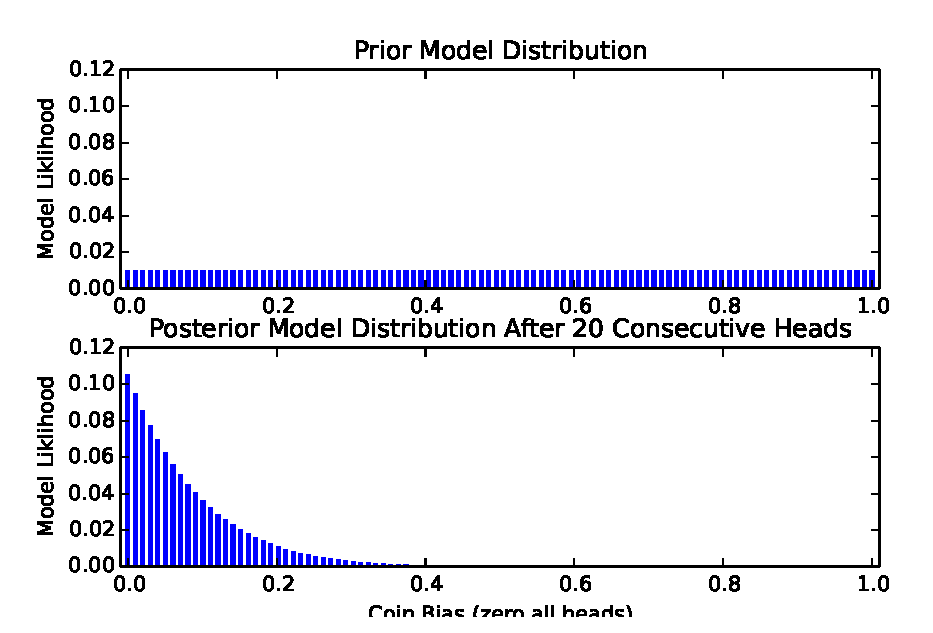
\includegraphics[scale=0.8]{Figures/bayes.eps}
\caption{Example prior and posterior distribution for a set of coin flip models that samples 10 heads flips in a row}
\label{fig:bayes}
\end{figure}
\subsection{Markov Chain Monte Carlo Methods}
\label{sec:mcmcupdate}
Often when attempting to fit a model it is computationally infeasible to explore the entire model space. This can be due to having a large number of possible models, models having a large number of parameters and the fact that most physical process parameters are described by real numbers and it is therefore impossible to explore the entire parameter space. A way to deal with model selection in this case is known are Markov Chain Monte Carlo (MCMC) methods. Given a set of models 
\begin{equation}
\mathcal{M} = \left\{\mathbf{M}(x_1,x_2,\cdots,x_i;y_1,y_2,\cdots,y_i) : y_j \in \mathcal{F}\right\}
\label{eq:models}
\end{equation}
where $x_j$ are input variables to the model and $y_j$ are model parameters, it is desired to find and approximate ideal model. MCMC methods will select an original set of possible model parameters $$\mathbf{P} = \left\{(y_{11},y_{12},\cdots,y_{1i}),\cdots,(y_{j1},y_{j2},\cdots,y_{ji})\right\}$$ and assign a prior distribution to these models $\mathcal{D}_{prior}$. Given a set of inputs $$\mathbf{I} = \left\{(x_{11},x_{12},\cdots,x_{1i}),\cdots,(x_{j1},x_{j2},\cdots,x_{ji})\right\}$$ the posterior distribution $\mathcal{D}_{pos}$ can be evaluated using (\ref{eq:discretebayes}). In order to explore the parameter space, the algorithm must select a new set of parameters. One method of doing this is to select some $\subset \mathbf{P}$ and generate a new set of models and posterior distributions according to some utility function\cite{bayes}
\begin{equation}
\mathcal{M}_{pos},\mathcal{D}_{pos_2} = f(\mathcal{M},\mathcal{D}_{pos})
\label{mcmcupdate} 
\end{equation}

It is useful to think of the set of selected model parameters as a large number of points in space, in practice these are often referred to as points. By re-sampling model parameters as in (\ref{mcmcupdate}) it is possible to select points throughout the parameter space and ideally zero in on the optimal model. However, due to the nature of sampling normally being non-deterministic and numerical precision errors, it is crucial to examine the convergence of the model to experimental data. 

\subsection{Fisher Information and the Cramer-Rao Lower Bound}
The Cramer-Rao lower bound is hugely important in statistics as it provides a lower bound on the variance of an unbiased estimator 
\subsubsection{Covariance Matrix}
The covariance matrix in statistics is a measure of how a random vector of variables changes together. Two random variables are related by their covariance $\sigma(x,y) = E_x \left[(x-E[x])(y-E[y])\right]$, where $E[x]$ denotes the expectation value of $x$. As an example, in quantum mechanics the expectation value according to the Born interpretation is as in (\ref{eq:quantumExpectation}). The covariance of two random variables can be generalized to that of a random vector of estimated coefficients $\mathbf{X}$ where \cite{covariance}
\begin{equation}
cov(\mathbf{X})_{ij} = cov(X_i,X_j) = E[(X_i-E[X_i])(X_j-E[X_j])]
\end{equation}
Which in matrix notation takes the form 
\begin{equation}
\mathbf{\Sigma} = cov(\mathbf{X}) = [(\mathbf{X}- u)(\mathbf{X}-u)^T] = E(\mathbf{X}\mathbf{X}^T) - uu^T
\label{eq:covarianceMatrix}
\end{equation}
Where $u=E(\mathbf{X})$. It is prudent to note that the elements of the diagonal of the covariant matrix $\sum{ii}$ are the variances of the elements of the vector $\mathbf{X}$. When $\sigma(x,y)>0$ the relationship between the two variables tends to be similar, ie. when one grows the other grows and similarly when $\sigma(x,y)<0$ when one variable grows the other will tend to show the opposite behaviour.\cite{covariance}  

\subsubsection{Cramer-Rao Lower Bound}
The Cramer-Rao lower bound states that the variance of an unbiased estimator $\hat{\theta}$ is lower bounded by the reciprocal Fisher Information $I(\theta)$.\cite{cramerrao} 
\begin{equation}
var(\hat{\theta}) \geq \frac{1}{I(\theta)}
\label{eq:cramerao}
\end{equation}
The Fisher Information is the expectation value of the square of the first moment of the log likelihood function for some probability density function $Pr(\mathbf{X};\theta)$. The log-likelihood of the probability density function is defined as $\mathcal{l}(\mathbf{X};\theta) = log(Pr(\mathbf{X};\theta))$
Therefore the Fisher information is 
\begin{equation}
I(\theta) = E\left[\left(\frac{\partial}{\partial \theta} log (Pr(\mathbf{X};\theta)) \right)^2 \Big| \theta \right] = -E\left[\frac{\partial^2}{\partial\theta^2} l(\mathbf{X};\theta) \Big| \theta \right]
\label{eq:fisherinformation}
\end{equation}
The Fisher Information is the variance of the statistical score of the probability density function. Geometrically it is a measure of the amount of curvature of the log-likelihood function. It is a measure of the amount of information an observable $\mathbf{X}$ carries about an unknown parameter $\theta$ of which the probability of $\mathbf{X}$ relies on according to the function $Pr(\mathbf{X};\theta)$. In multiple dimensions the Fisher Information matrix takes the form 
\begin{equation}
\mathbf{I}(\mathbf{\theta}) = E_D[\mathbf{\nabla}_\mathbf{\theta}log(P(D|\mathbf{\theta}))\cdot \mathbf{\nabla}^T_\mathbf{\theta}log(P(D|\mathbf{\theta}))]
\label{eq:fishermatrix}
\end{equation}

The Cramer-Rao lower bound establishes a lower limit on the amount of information an unknown parameter of a probability distribution carries.\cite{cramerrao2} This is very useful in determining the fit of a set of model parameters as shall be seen. It is important to keep in mind that this only holds for unbiased estimators and may be violated by biased estimators. 

\section{Robust Online Hamiltonian Learning}
\label{sec:robusthamiltonian}
The construction of a large scale quantum information processor is an extremely difficult challenge. Before error correcting codes and algorithms can be applied to such a system, the full characterization of the system is required. This is normally achieved via statistical estimation of Hamiltonian parameters via tomography. In quantum tomography the process is normally carried out on the device as a \textit{black box} and a set of measurements is chosen such that the parametrization of them will allow the output of any input state to be predicted.\cite{tomography} Full tomography is computationally complex and requires the simulation of the behaviour of the quantum system. As the systems being simulated grow in complexity, it is no longer possible for classical computer to simulate.\cite{simulate}

In practice there is often more information available about the form of the Hamiltonian of a given system and this allows the number of parameters that need be estimated to be reduced. This is known as partial process estimation or partial tomography. The goal of the experiment proposed in this thesis is to provide experimental verification of the algorithm proposed in the 2013 paper "Robust Online Hamiltonian Learning" by Chris Granade at the University of Waterloo.\cite{hamiltonian_learning} 

An additional benefit to the algorithm of focus is that in quantum mechanics, often future measurement results depend on prior measurements. The use of MCMC methods allows model parameters to be estimated for such time dependent measurements. As given a set of estimated models for the hamiltonian it is possible to predict the probability of a future measurement $d_{N+1}$ given a future set of experimental controls $c_{N+1}$. 
\begin{equation}
P(d_{N+1}\big|D;c_{N+1},C) = E_{\mathbf{x}|D;C}[P(d_{N+1}\big|\mathbf{x};c_{N+1}]
\label{eq:batch}
\end{equation}

\subsubsection{Algorithm Specifics}
\subsubsection{Bounding the Error of an Estimator}
Given a set of future experimental controls and their potential outcome probabilities it is useful to quantify the measurements usefulness. This is just the utility function as described in section (\ref{sec:mcmcupdate}). An often used measure is that of information gain, or in other words the expectation value of the logarithm of the estimator. 
\begin{equation}
U(d_{N+1};c_{N+1}) = E_{\mathbf{x}|d{N+1},D;c_{N+1},C}[log Pr(\mathbf{x}|d_{N+1},D;c_{N+1},C)]
\label{eq:utilityfunction}
\end{equation}
Maximizing the utility function is equivalent to minimizing the entropy of the posterior distribution.

The quality of an estimator $\mathbf{\hat{x}}$ for a set of observed data $D$ and experimental controls $C$ can be quantified by using the quadratic loss function 

\begin{equation}
L_{\mathbf{Q}}(\mathbf{x},\mathbf{\hat{x}}(X,X)) = (\mathbf{x},\mathbf{\hat{x}}(D,C))^T\mathbf{Q}(\mathbf{x},\mathbf{\hat{x}}(D,C))
\label{eq:quadraticloss}
\end{equation}
Where $\mathbf{Q}$ is a chosen positive definite matrix deciding the importance of model parameters in the quadratic loss function. The quadratic loss is used to define the risk of an estimator by taking the expectation value of the quadratic loss over all possible outcomes of the experiment.
\begin{equation}
R(\mathbf{x},\mathbf{\hat{x}};C) = E_{D|\mathbf{x};C}[L(\mathbf{x},\mathbf{\hat{x}}(D,X))]
\label{eq:risk}
\end{equation}
The Bayes' risk is the average risk of the risk function with respect to a prior distribution $\pi(\mathbf{x})$
\begin{equation}
r(\pi;C) = E_\mathbf{x}[R(\mathbf{x},\mathbf{\hat{x}};C)] = \int \pi(\mathbf{x})R(\mathbf{x},\mathbf{\hat{x}};C)d\mathbf{x}
\label{eq:bayesrisk}
\end{equation}
Here $\mathbf{\hat{x}}$ is taken to be the unique Bayes' estimator, which is the estimator that minimizes the total risk. The utility function is chosen as the negative Bayes' risk as this corresponds to minimizing the Bayes' risk for chosen set of parameters. 
 
Remembering the Fisher information matrix as defined in (\ref{eq:fishermatrix}) we call the Bayesian information matrix\cite{bayesiancramer}
\begin{equation}
\mathbf{J}(\pi;C) = E_\mathbf{x}[\mathbf{I}(\mathbf{x};C)] = \int \pi(\mathbf{x})R(\mathbf{x},\mathbf{\hat{x}},C)d\mathbf{x}
\label{eq:bayesianinformation}
\end{equation}
From Bayesian information matrix a lower bound on the risk function called the Bayesian Cramer-Rao bound can be placed \cite{bcrb}
\begin{equation}
\label{eq:bayeslowerbound}
r(\pi;C)\geq \frac{1}{\mathbf{J}(\pi;C)}
\end{equation}

This is used rather than the Fisher Information as in the case of an experiment giving no information about a parameter set, the Fisher Matrix $I$ is singular and therefore its inverse is undefined, this is resolved via the Bayesian Cramer-Rao Lower Bound (\ref{eq:bayeslowerbound}). 

Given (\ref{eq:bayeslowerbound}) the lower bound on the Bayes' risk can be iteratively monitored. 
\begin{equation}
r(\pi;C_{N+1})\geq \frac{1}{\mathbf{J}_{N+1}(C_{N+1})}
\end{equation}
where 
\begin{equation}
\mathbf{J}_{N+1}(C_{N+1} = \mathbf{J}(\pi;C_{N+1})+ J_N(C_N)
\label{eq:riskiteration}
\end{equation}
\subsubsection{Resampling}
\label{sec:resampling}
Utilizing sequential Monte Carlo methods the costly posterior distribution are approximately calculated by approximating the distribution as a set of particles or points distributed over the parameter space, each with weight $w_i$ and with the sum of all weights being $\sum \limits_i w_i = 1$. Therefore the probability distribution is 
\begin{equation*}
Pr(\mathbf{x}|D) \approx \sum \limits_{k=1}^n w_k(D)\delta(\mathbf{x}-\mathbf{x}_k)
\end{equation*}
with the weights being iteratively updated according to 
\begin{equation*}
w_k(d_{j+1} \cup D) = \sum \limits_{k=1}^n P(d_{j+1}|\mathbf{x}_k)w_k(d_j)
\end{equation*}
As with MCMC algorithms the accuracy can be made arbitrarily high by increasing the number of particles. The initial weights are chosen to simply be $w_k = 1/n$. Using this approximate distribution, Bayes' updates can be performed and an accurate estimator approached.

Since any particle estimate will only ever approach the true parametrization, all weights will tend to zero. This can be postponed by re-sampling and updating weights at intervals. The basic idea is too select some $n$ most likely particles and choose new particles around these likely particles according to some distribution to replace unlikely particles. Re-sampling will be performed when $n_ess = 1/\sum \limits_i w_i^2>0.5$ where $0.5$ is the re-sampling threshold. After re-sampling the weights are reset. 

The algorithm to be tested adds the additional step of a random normally distributed perturbation vector $\mathbf{\epsilon}= \mathcal{N}(0,\sum \limits)$ to the position of a random selected point. This is to further increase the size of the parameter space explored.\cite{hamiltonian_learning}
\begin{equation}
pos(\mathbf{x'}) = \sum \limits_i w_i \frac{1}{\sqrt{(2\pi)^k|\sum|}}exp\left(-\frac{1}{2}(\mathbf{x'}-\mathbf{u_i})^T\mathbf{\Sigma}^{-1}(\mathbf{x'}-\mathbf{u_i})\right)
\label{eq:resample}
\end{equation}
Where $k$ is the number of model parameters. This distribution is known as a mixture distribution. The mean $u_i$ of each particle is chosen using a linear combination of the form 
\begin{equation}
\mathbf{u}_i = a\mathbf{x}_i + (1-a)\mathbf{u}
\end{equation}
Where $\mathbf{u}= E[\mathbf{x}]$. Therefore re-sampling consists of sampling from the distribution described by (\ref{eq:resample}) for the $k=N-n$ unselected particles and then resetting all weights to $w_i = 1/n$.  
\subsubsection{Region Estimation}
\label{sec:regionestimation}
It is not just important to have an accurate estimator for the system, but also crucial to be able to quantify the error in the estimator and how much it differs from the  Bayesian Cramer-Rao lower bound. This is achieved by finding a region of the parameter space $\mathbf{\hat{X}}$ such that the probability of the true parameter set $\mathbf{x_0}$ is contained within $\mathbf{\hat{X}}$ is maximized, while the volume $V(\mathbf{\hat{X}})$ is minimized.\cite{hamiltonian_learning}

The probability of the true model being within a region $\mathbf{\hat{X}}$ can be expressed as 
\begin{equation}
Pr(\mathbf{x_0}\in \mathbf{\hat{X}}) = E[1_{\mathbf{\hat{X}}}]
\end{equation}
Where $1_{\mathbf{\hat{X}}}(x) = 1$ if $\mathbf{x}\in \mathbf{\hat{X}}$ and otherwise $1_{\mathbf{\hat{X}}}(x) = 0$. 
The probability of a region can then be calculated from the particle weights from section (\ref{sec:resampling}). 
\begin{equation}
E[1_{\mathbf{\hat{X}}}] \approx \sum \limits_i w_i 1_{\mathbf{\hat{X}}}(\mathbf{x}_i) = \sum \limits_{i,\mathbf{x_i}\in\mathbf{\hat{X}}} w_i
\label{eq:probin}
\end{equation}
Therefore a region $\mathbf{\hat{X}}$ must be found such that (\ref{eq:probin}) is sufficiently large, while $V(\mathbf{\hat{X}})$ is sufficiently small. Under the assumption that after a reasonable amount of data the posterior distribution is approximately normally distributed according to $\mathcal{N}(\mathbf{\mu},\mathbf{\Sigma})$, from the definition of the normal distribution it follows that the inverse covariance matrix $\Sigma^{-1}$ describes an ellipse of dimension $d$ where $0.682^d$ of the probability mass is contained within the ellipse. Where, $d$ is the number of model parameters. 
The volume of the ellipse can be found to be 
\begin{equation}
V(\mathbf{\Sigma^{-1}}) = \frac{\pi^{d/2}}{\Gamma(d/2+1)}det(\mathbf{\Sigma^{-1}}) 
\end{equation}
In order to determine the fit of the region found, it is important to compare the found covariance ellipse to the optimal one according to the Bayesian Cramer-Rao lower bound 
\begin{equation*}
E_\pi [cov(\mathbf{\hat{x}})] \geq \mathbf{J}(\pi;C)^{-1}
\end{equation*}
\section{Experimental Verification of the Robust Online Hamiltonian Learning Algorithm}
While simulations predict that the algorithm introduced in sec(\ref{sec:robusthamiltonian}) quickly approaches the lower bound on the error for a variety of physical systems.\cite{hamiltonian_learning} It has yet to be verified experimentally. Therefore a proof of concept neutron interferometry experiment will be proposed which theoretically should allow the prediction of neutron interferometer model parameters and improve the maximum contrast of interferometer measurements. As control of the contrast of the neutron interferometer is desired, precise contrast control will only be obtainable when all system parameters are known. 
\subsection{Experimental Model}
Take the O and H detectors as 0 and 1 respectively. We model the probability of the neutron striking the $O$ detector similarly to (\ref{eq:normalizedIntensities}) except now the model is non-ideal and has parameters that must be fitted to it as 
\begin{equation}
P(0|A,b,\delta\phi,C,\delta) = (\frac{1}{2}+b) + \frac{A}{2}cos(\Delta\phi+C\delta)
\label{eq:model1}
\end{equation}
where $b$ is an unknown experimental offset,$A$ is an unknown amplitude, $\Delta\phi$ is the induced phase due to the different paths, $C$ is the phase flag constant and $\delta$ is the phase flag setting. 
\subsubsection{Humidity and Temperature Phase Dependence}
As the neutron interferometry chamber is not humidity or temperature controlled we will attempt to increase the contrast of measurements by accounting for the induced phase shift due to the water vapour in the air. This phase shift will occur if there is a path length difference between the two interferometer paths. This path length difference will be induced by one of the paths spending a longer time in the phase flag and therefore will be a function of the phase flag angle. The model will now have the form 
\begin{equation}
P(0|A,b,\Delta\phi,C;\delta) = (\frac{1}{2}+b) + \frac{A}{2}cos(\Delta\phi+C\delta+\Delta\gamma(\Phi,T,\delta))
\end{equation}
Where 
\begin{equation*}
\Delta\gamma(\Phi,T,\delta) = \frac{n}{v}\lambda b D
\end{equation*}
$D$ is the path length difference and from sec(\ref{sec:phaseflag}) the phase shift as a function of the phase flag angle is the negative of (\ref{eq:relative_phase}) due to the extra path length in the water vapour occurring when the other pass is still in the phase flag. therefore the phase difference induced by the water vapour is 
\begin{equation}
\Delta\gamma(\Phi,T,\delta)= 2\frac{n(\Phi,T)}{V}b_{water}\lambda D\frac{sin(\theta_B)sin(\delta)}{cos^2(\theta_B)-sin^2(\delta)} \approx \alpha \times \frac{n(\Phi,T)}{V}\delta 
\label{eq:phasewater}
\end{equation}
Where $\alpha$ is the phase multiplier constant and $\delta$ is the angle of the phase flag.

By the ideal gas law 
\begin{equation}
\frac{n(\Phi,T)}{V} = \frac{p_w(\Phi,T)}{RT}
\end{equation}
The partial pressure of water $p_w$ at percent humidity $\Phi$ is given by 
\begin{equation}
p_w(\Phi,T) = \Phi p^*_w(T)
\label{eq:partialPressure}
\end{equation}
Where $p^*_w$ is the saturation vapour pressure in bars.\cite{relativehumidity} The saturation pressure of water at temperature $T$ can be fitted to the Antoine equation \cite{antoineequation}
\begin{equation}
\label{eq:antoine}
p^*_w(T) = 10^{h_A - \frac{h_B}{h_C + T}}
\end{equation} 
Therefore $h_A,h_B$ and $h_C$ are empirical constants that must be fitted and are parameters of the estimator for the $O$ detector model. In the range of $255.9K-373K$ the parameters were fitted to values $h_A=6.20963$,$h_B=2354.731$ and $h_C=7.559$.\cite{antoineequation} 
\begin{figure}[ht!]
\centering
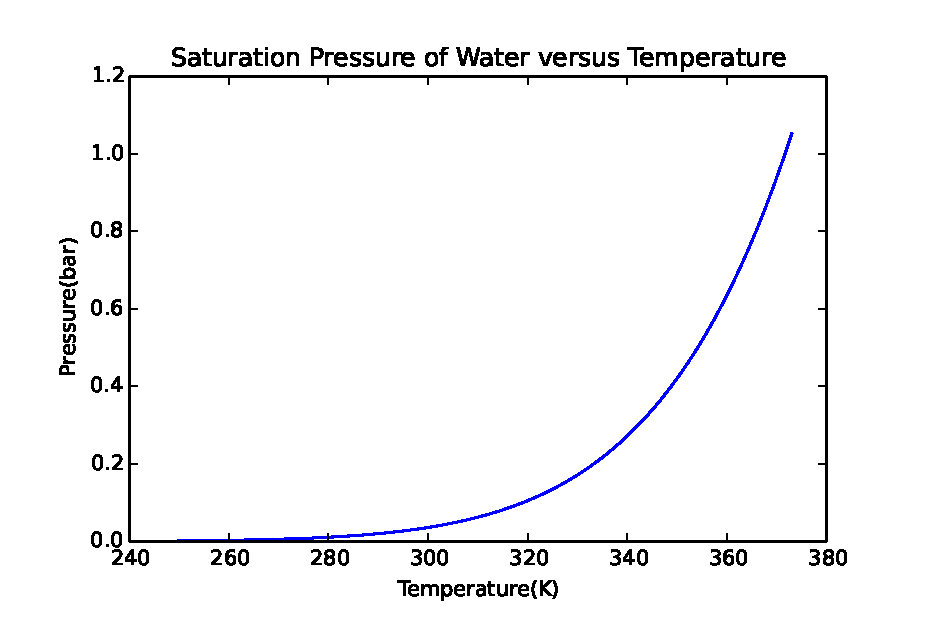
\includegraphics[scale=1.0]{Figures/antoine.eps}
\caption{Saturation Pressure as a function of temperature}
\label{fig:antoine}
\end{figure}
The phase shift due to water vapour is can be found by combining (\ref{eq:phasewater}),(\ref{eq:partialPressure}) and (\ref{eq:antoine}) to obtain
\begin{equation}
\Delta\gamma(\Phi,T,\delta) = \frac{\alpha'\Phi\delta}{T}\times 10^{h_A - \frac{h_B}{h_C - T}}
\label{eq:phasewaterfinal}
\end{equation}
In reality we do not have the exact values of $\Phi$ and $T$ and therefore must marginalize over the distribution of $P(T,\Phi|\hat{T},\hat{\Phi})$ conditioned on the estimator for the phase shift described by (\ref{eq:phasewaterfinal}).
\begin{equation}
Pr(\Delta\gamma|\hat{\Phi},\hat{T})= \int \limits_\Phi \int \limits_T Pr(\Delta\gamma|\Phi,T)P(T,\Phi|\hat{T},\hat{\Phi})dTd\Phi
\label{eq:marginalizeprop}
\end{equation}  
For simplicity we assume that $\hat{\Phi}\perp\hat{T}$ which reduces 
(\ref{eq:marginalizeprop}) to 
\begin{equation}
Pr(\Delta\gamma|\hat{\Phi},\hat{T})= \int \limits_\Phi \int \limits_T Pr(\Delta\gamma|\Phi,T)P(T,\hat{T})Pr(\Phi,\hat{\Phi})dTd\Phi
\label{eq:marginalizeprop2}
\end{equation}
Taking account of the humidity and temperature dependence of the phase due to water vapour in the air, the updated model now takes the form 

\begin{equation*}
  P(0|A,b,\Delta\phi,C,\alpha';\delta,\hat{\Phi},\hat{T}) = \int \limits_{\Delta\gamma} P(0|A,b,\Delta\phi,C,\delta,\alpha',\hat{\Phi},\hat{T},\Delta\gamma)d\Delta\gamma =
\end{equation*}
\begin{equation*}
= \int \limits_{\Delta\gamma} \int \limits_\Phi \int \limits_T P(0|A,b,\Delta\phi,C,\alpha';\delta,\Phi,T,\Delta\gamma)P(T,\hat{T})Pr(\Phi,\hat{\Phi})dTd\Phi d\Delta\gamma =
\end{equation*}
\small
\begin{equation}
= \int \limits_\Phi \int \limits_T \left[(\frac{1}{2}+b)+\frac{A}{2}cos\left(\Delta\phi + C\delta + \frac{\alpha' \Phi\delta}{T}\times 10^{h_A - \frac{h_B}{h_C + T}}\right)\right]P(T|\hat{T})Pr(\Phi|\hat{\Phi})dTd\Phi
\label{eq:finalmodel}
\end{equation}
\normalsize
The integral in (\ref{eq:finalmodel}) will be integrated using Monte Carlo sampling techniques in order to reduce the computational complexity involved in evaluating (\ref{eq:finalmodel}) many, many times. Provided the temperature and humidity data is normally distributed the required number of samples should be $n\approx100-300$ and is tunable based on the desired accuracy. Similarly to the original model (\ref{eq:model1}), due to the small angle approximation of the phase flag a lower bound must be put on the phase induced by the flag and water vapour, in order to allow full phase control. 
\begin{equation}
C+\frac{\alpha'\Phi}{T}\times 10^{h_A - \frac{h_B}{h_C + T}} \geq 20
\label{eq:fullphasecontrol}
\end{equation}

\subsection{Model Analysis}
Due to unforeseen departmental issues it was not possible to experimentally verify the model (\ref{eq:finalmodel}) using the algorithm described in sec(\ref{sec:robusthamiltonian}). However it was possible to simulate the model for test \textit{true} parameters and simulate both naive and adaptive experiments to determine if it should be possible to reduce the Bayes' risk to an acceptable level. A variety of \textit{true} parameter sets were chosen, to test the affects of different parameters as seen in table (\ref{tab:trueparams}). 
\begin{table}[h]
\begin{center}
\begin{tabular}{l*{6}{c}r}
Parameter Set     & A&b& $\Delta\phi$ & C & $\alpha$ & Description \\
\hline
1& 0.9& 0.0& 0.0844& 22.02& -1.02 & Normal set of Parameters  \\
2&  0.9& 0.0& 0.0844& 15.0& -1.02 & No full phase control \\
3& 0.9& 0.0& 1.5707& 22.02& -1.02 &   Larger phase offset \\
4& 0.7& 0.0& 0.0844& 22.02& -1.02 & Smaller A constant\\
5& 0.1& 0.0& 0.0844& 22.02& -1.02 & Very small A constant\\
6&  0.7& 0.1& 0.0844& 22.02& -1.02 & B is offset\\
\end{tabular}
\caption{True parameter sets to simulate model for}
\label{tab:trueparams}
\end{center}
\end{table}
In fig(\ref{fig:likelihoods}) the likelihood of detection at the O-detector for the system parameters in table (\ref{tab:trueparams}) are plotted as a function of the phase flag angle $\delta$ at a temperature of $293.15K$ and humidity of $70\%$. 

\begin{figure}[ht!]
\centering
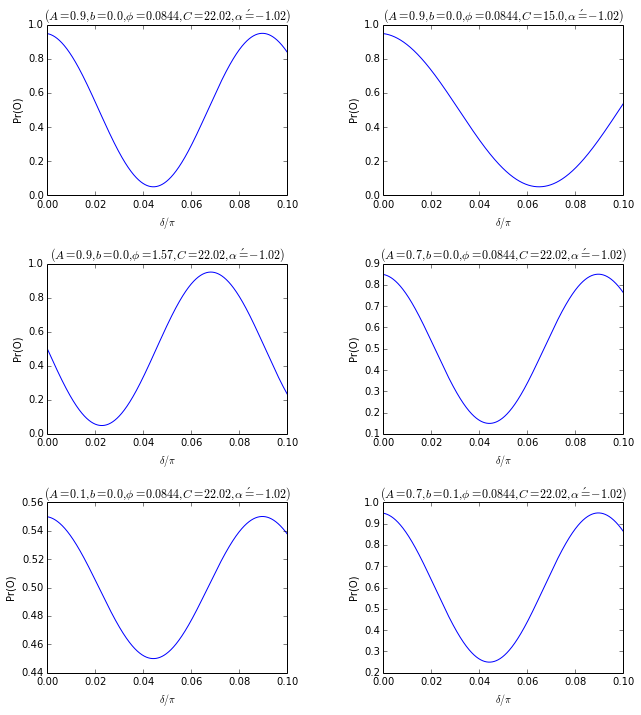
\includegraphics[scale=0.7]{Figures/likelihoods.png}
\caption{Liklihood of detection at O-detector for various system parameters as a function of $\delta$, $T=293.15$,$\Phi=70\%$}
\label{fig:likelihoods}
\end{figure}

It can be seen that the likelihood of detection is never $100\%$ due to the parameter $A$ being less one in all test cases. In the case of parameter set five, $A$ is very small and the result is a very low maximum probability of detection. Additionally, in the case of parameter set 2 it can be seen that full phase control does not exist due to the weakness of the settings of the phase flag constant $\alpha'$.   Uniform prior distributions were established around the true values as in table (\ref{tab:around}). The set of starting values were kept relatively near to the true values in order to reduce simulation time. It should be noted that the specifications of the system that the simulations were performed on can be found in appendix (\ref{app:testsystem}). 
\begin{table}[h]
\begin{center}
\begin{tabular}{l*{5}{c}r}
A&b& $\Delta\phi$ & C & $\alpha$ \\
\hline
 $\pm0.02$ & $\pm0.02$ & $[0,\frac{pi}{2}]$ & $\pm0.05$ & $\pm0.05$
\end{tabular}
\caption{Range around true parameters that prior distributions were established for}
\label{tab:around}
\end{center}
\end{table}
From these initial uniform distributions the Bayes' risk can be calculated as seen in fig(\ref{fig:initialdistributions}).
\begin{figure}[ht!]
\centering
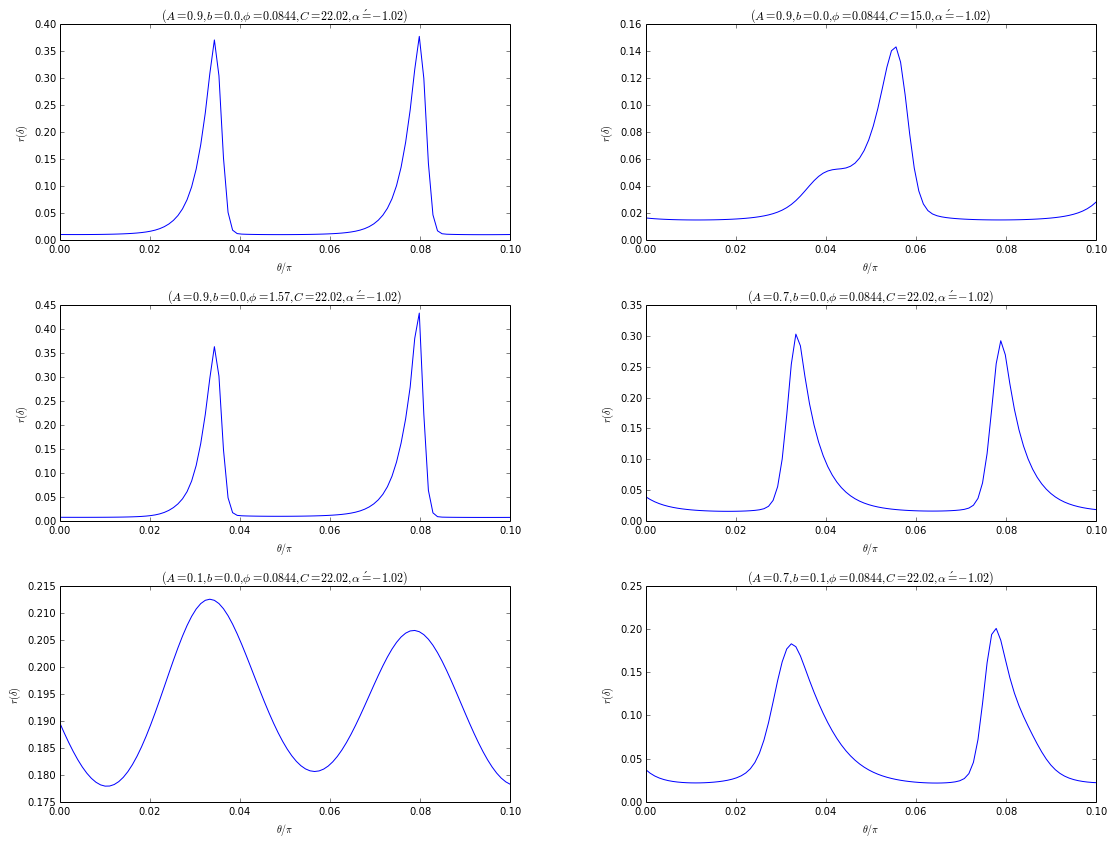
\includegraphics[width=\textwidth , height=0.8\textheight]{Figures/priors.png}
\caption{The Bayes' Risk of the initial prior distributions}
\label{fig:initialdistributions}
\end{figure}
It is clear that the initial risk is very large. This is as to be expected since the initial distributions are simply uniform distributions. It should be noted that the risk is largest around the point when the sum of the phases is $\pm\pi/2$. This is because when the total phase offset is $\pm\pi/2$, $cos(\pi/2)=0$ and there is no information about any parameters except $b$. The risks of parameter set two are singularly peaked, due to the lack of full phase control. 

We next examine the algorithm behaviour for an experiment in which $2^15$ linearly spaced values for $\delta$ from $\delta=[0,\pi/10]$ are measured, with the assumption that at each interval $100$ neutrons are detected. The Monte Carlo algorithm is using $20000$ particles. Additionally the temperature is set to $293.15\pm0.5K$ and the humidity $70\pm1\%$, both are normally distributed. While this experiment is unrealistic as the number of neutrons detected would be much larger than $100$ and would be varying, it serves as a naive simulation. The results are as seen in fig(\ref{fig:naiverisks}). 
\begin{figure}[ht!]
\centering
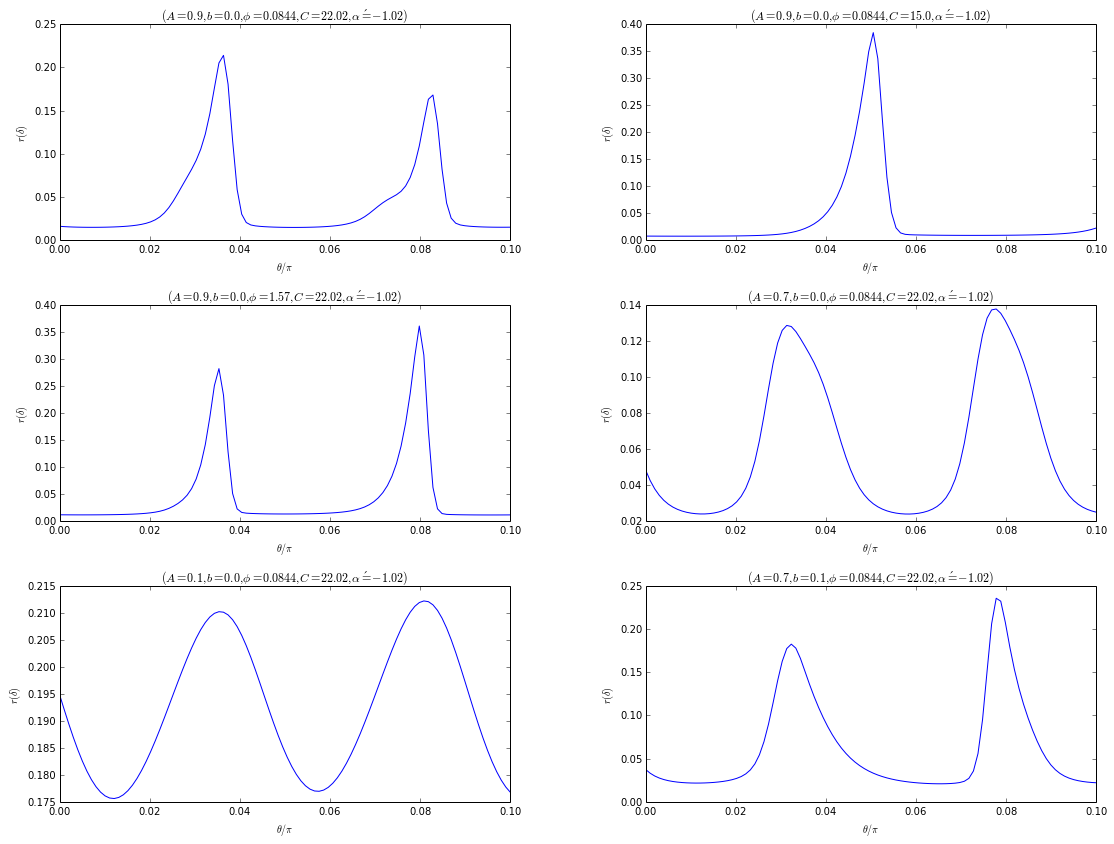
\includegraphics[width=\textwidth , height=0.8\textheight]{Figures/naiverisk.png}
\caption{Approximate calculated system parameters from naive experiment with $2^{15}$ linearly spaced phase flag angles $0<\delta<\pi/10$.}
\label{fig:naiverisks}
\end{figure}
From the naive simulation it can be seen the risk is over two to three orders of magnitude lower than that of the uniform distribution for all parameter sets. Additionally, the risk is much more uniform in value over the entire phase flag range as all risks fluctuate only by order $10^-7$. The approximate values for the system parameters calculated by the simulation can be found in table (\ref{tab:naiveparams}). From the calculated parameters it is clear to see that almost all parameters are properly calculated within one to two standard deviations of error. Therefore we can conclude that given enough measurements the algorithm will converge on the correct model parameters, at least in theory.

\begin{table}[h]
\tiny
\begin{center}
\begin{tabular}{l*{5}{c}r}
Parameter set & A&b& $\Delta\phi$ & C & $\alpha$ \\
\hline

1 &$0.9007 \pm 0.0004$&$	 0.0005 \pm 0.0002$&  $0.087 \pm 0.002$ & $22.009 \pm 0.009$	& $-1.0225 \pm 0.026762$	\\

2& $0.9004 \pm 0.0007$ &	 $0.0003 \pm 0.0004$	&$0.084 \pm 0.003$	& $15.00 \pm 0.01$ & $-1.01 \pm 0.03$	\\

3&$0.8999 \pm 0.0005$ &	 $0.0004 \pm 0.0002$	& $1.5687 \pm 0.0009$& $22.029 \pm 0.006$ & $-1.02 \pm 0.03$	\\

4&$0.7010 \pm 0.0006$ &	 $0.0000 \pm 0.0003$	 &$0.084 \pm 0.002$	& $22.02 \pm 0.01	$ & $-1.0093 \pm 0.027575$	\\

5&$0.0995 \pm 0.0008$ &	$0.0003 \pm 0.0003$ &	 $0.094 \pm 0.009$	& $22.02 \pm 0.03$	 &$-1.02 \pm 0.03$	\\

6&$0.7000 \pm 0.0005$ &	 $0.0996 \pm 0.0003$	 &$0.084 \pm 0.002$	& $22.04 \pm 0.01$ &	 $-1.02 \pm 0.03$	\\

\end{tabular}
\caption{Approximate calculated system parameters from naive experiment}
\label{tab:naiveparams}
\end{center}
\end{table}

While the experiment simulated above is simply a parameter sweep of as many $\delta$ values as possible, the import feature of the tested algorithm is experimental design. By simulating future experiments based on the present probability distributions it is possible to select experimental parameters such that the information gain is maximized and the Bayes' risk minimized. The results of the adaptive simulations can be seen in fig(\ref{fig:adaptiverisks}). Note that the risk is very low in comparison to the naive simulation. An interesting aspect to note is that the two simulations with the most extreme system parameters, parameter sets two and five, demonstrate very jagged risk curves. This is most likely due to the inability to adequately choose experimental parameters when the ability to control the system is small such as in these two cases. 
\begin{figure}[ht!]
\centering
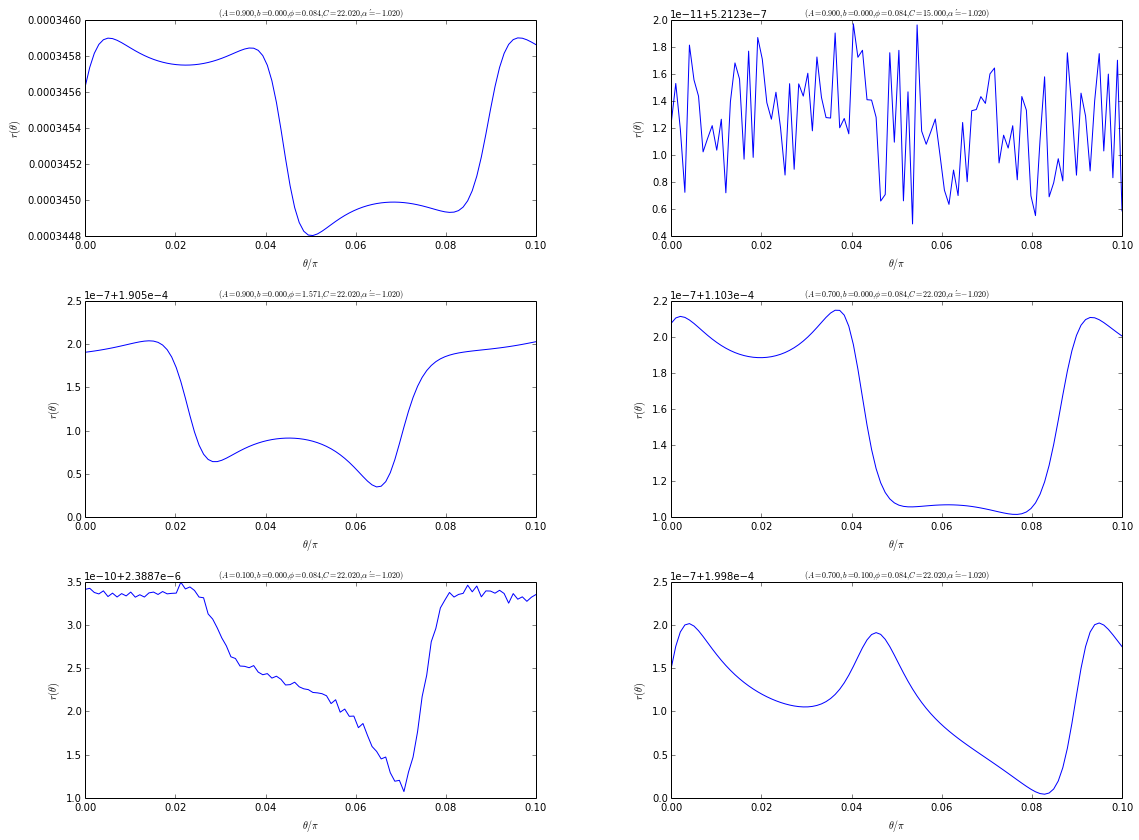
\includegraphics[width=\textwidth , height=0.8\textheight]{Figures/adaptiverisk.png}
\caption{The Bayes' Risk from an adaptive simulations, when 200 experiments were performed with experimental parameters chosen to maximize the information gain.}
\label{fig:adaptiverisks}
\end{figure}

\begin{table}[h]
\tiny
\begin{center}
\begin{tabular}{l*{5}{c}r}
Parameter set & A&b& $\Delta\phi$ & C & $\alpha$ \\
\hline
1&$0.901\pm 0.006	$& $0.000 \pm 0.004$&$	 0.09 \pm 0.02	$&$ 22.000 \pm 0.006$&$	 -1.020 \pm 0.006$\\	

2&$0.8896 \pm 0.0002	$&$ -0.0080 \pm 0.0001	$&$ 0.0150 \pm 0.0002	$&$ 22.0130 \pm 0.0003$&$ -1.0227 \pm 0.0006$\\

3&$0.901 \pm 0.006	$&$ -0.005 \pm 0.003	$&$ 1.554 \pm 0.009	$&$ 22.001 \pm 0.006	$&$ -1.020 \pm 0.006	$\\

4&$0.894 \pm 0.001$&$	 -0.006 \pm 0.002	$&$ 0.273 \pm 0.009$&$	 22.002 \pm 0.003	$&$ -1.021 \pm 0.003$	\\

5&$0.8905 \pm 0.0004 $&$0.0137 \pm 0.0004	$&$ 1.196 \pm 0.001$&$	 22.0160 \pm 0.0004	$&$ -1.0141 \pm 0.0003	$\\

6&$0.894 \pm 0.004	$&$ 0.011 \pm 0.002 $&$	 0.04 \pm 0.01 $&$22.000 \pm 0.006	$&$ -1.018 \pm 0.006$\\
\end{tabular}
\caption{Approximate calculated system parameters from adaptive experiment with 200 adaptively chosen experimental parameters.}
\label{tab:adaptivedparams}
\end{center}
\end{table}
The parameters chosen for the acceptable system parameters can be seen in table (\ref{tab:adaptivedparams}). While close to the true system parameters in table (\ref{tab:trueparams}), they are not as close as those of the naive system as seen in table (\ref{tab:naiveparams}). This is very interesting considering the risk of the adaptive experiment is much lower. This is explained by the fact that the risk only provides a lower bound on the error in the experiment, it does not provide the true error. As the adaptive experiment actively attempts to minimize risk, it does not completely correlate with a minimization of absolute error. However as can be seen from the results it does function well in this regard too as the adaptive simulation only simulates $200$ experiments, whereas the naive simulation, simulates $2^{15}=32768$ experiments. If instead the adaptive experiment is compared against the case of $200$ naive experiments, it can be seen in fig(\ref{fig:naive200}) that the risks are much higher than the adaptive measurements which as expected. Additionally it can be seen in table (\ref{tab:naive200}) that the values selected by the algorithm as system parameters are much farther off and with large standard deviations than that of the adaptive algorithm. It is clear the adaptive experiment design is superior in terms of converging on the system parameter set in the least amount of experiments. 

\begin{figure}[ht!]
\centering
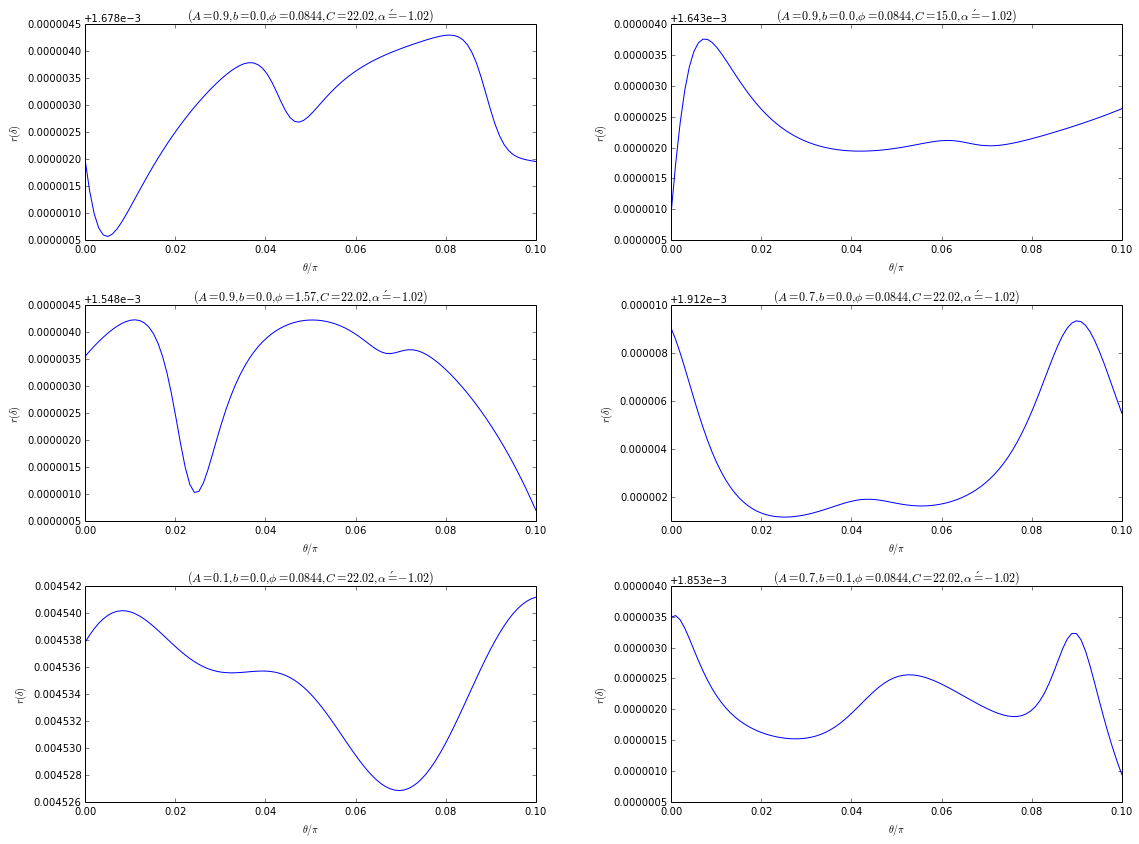
\includegraphics[width=\textwidth , height=0.8\textheight]{Figures/naive200.png}
\caption{The Bayes' Risk from a naive simulation, when 200 experiments were performed with linear space parameters from $0<\delta<\pi/10$.}
\label{fig:naive200}
\end{figure}
\begin{table}[h]
\tiny
\begin{center}
\begin{tabular}{l*{5}{c}r}
Parameter set & A&b& $\Delta\phi$ & C & $\alpha$ \\
\hline

1&$0.893 ± 0.005$&$	 -0.002 ± 0.002	$&$	 0.09 ± 0.01	 22.02 ± 0.03	$&$	 -1.02 ± 0.03$\\

2&$0.899 ± 0.007	$&$	 -0.001 ± 0.003$&$		 0.07± 0.01	$&$	 15.00 ± 0.03	$&$	 -1.01 ± 0.03$\\	

3& $0.900 ± 0.006$&$		 0.000 ± 0.002	$&$	 1.553 ± 0.008$&$	 22.01 ± 0.03$&$	 -1.01 ± 0.03$ \\	

4&$0.704 ± 0.007	$&$	 -0.003 ± 0.003	$&$	 0.08 ± 0.01	$&$	 22.02 ± 0.03	$&$	 -1.02 ± 0.03$ \\

5&$0.105 ± 0.008	 $&$	0.002 ± 0.003$&$		 0.08 ± 0.05	 $&$	22.02 ± 0.03	$&$	 -1.02 ± 0.03$ \\

6&$0.707 ± 0.006	$&$	 0.099 ± 0.003	$&$	 0.10 ± 0.01	$&$	 22.01 ± 0.03$&$		 -1.02 ± 0.03$\\	

\end{tabular}
\caption{Approximate calculated system parameters from naive experiment with 200 linearly spaced phase flag angles $0<\delta<\pi/10$.}
\label{tab:naive200}
\end{center}
\end{table}
It is interesting to observe how the error in the system parameters behave as additional experiments are performed. This can be seen in fig(\ref{fig:errexp}) for the error in the phase shift of $\Delta\phi$. It can be observed that the error rapidly decreases as the first experiments are performed and the algorithm gains information about the system. The error continues to decrease with additional experiments and tends to follow the Cramer-Rao Lower Bound for the simulation quite closely. 
 \begin{figure}[ht!]
\centering
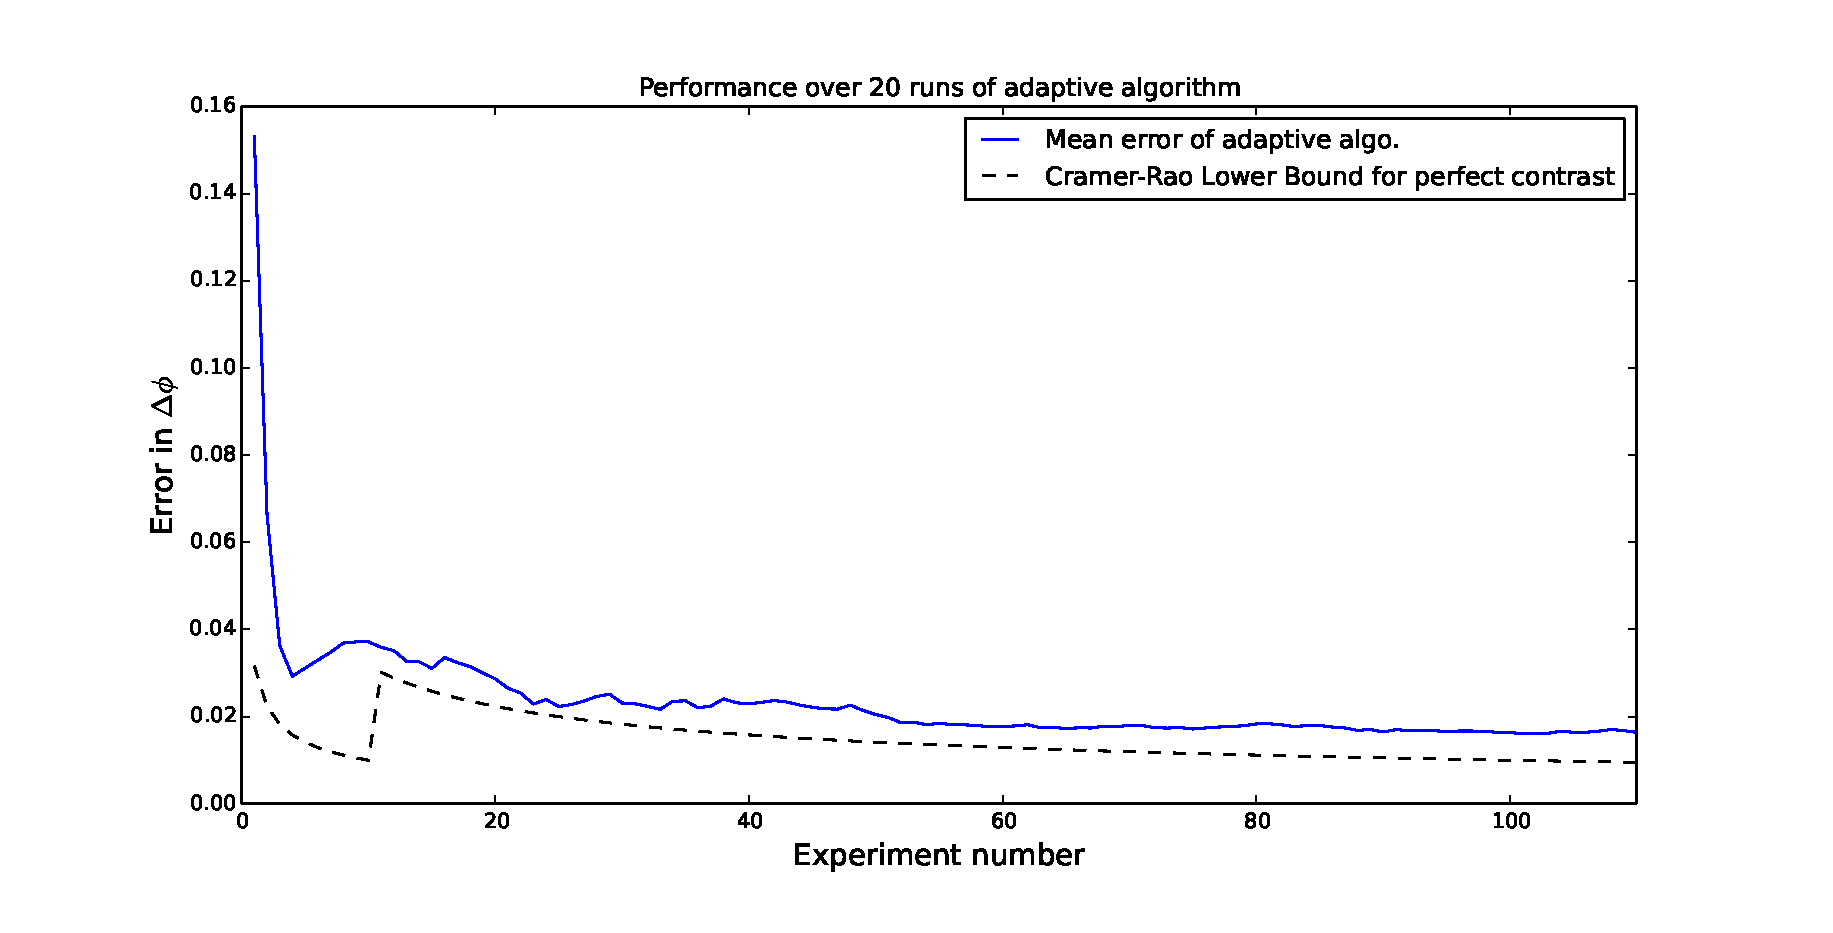
\includegraphics[width=\textwidth]{Figures/meanerror.eps}
\caption{The behaviour of the error in $\Delta\phi$ as additional experiments are performed, compared to the Cramer-Rao Lower Bound for the simulation.}
\label{fig:errexp}
\end{figure}
While the adaptive simulation does converge on the true system parameters much more quickly than that of the naive experiment, there are very real compromises. As can be seen in fig(\ref{fig:adaptivetimes}) the time taken to perform each adaptive measurement is many orders of magnitude larger than that of simply naively choosing experiments spread out over a range of experimental parameters. The choice to use adaptive measurements becomes a balancing act. Each adaptive experiment should provide more information than the naive experiments, however if the simulation time is much larger than the time it would take to perform many naive experts, it may not be efficient to use adaptive experiment design. However there are often ways of accelerating computation with an example explored in section (\ref{sec:gpu}), whereas normally it is quite difficult to speed up physical experiments.  
 \begin{figure}[ht!]
\centering
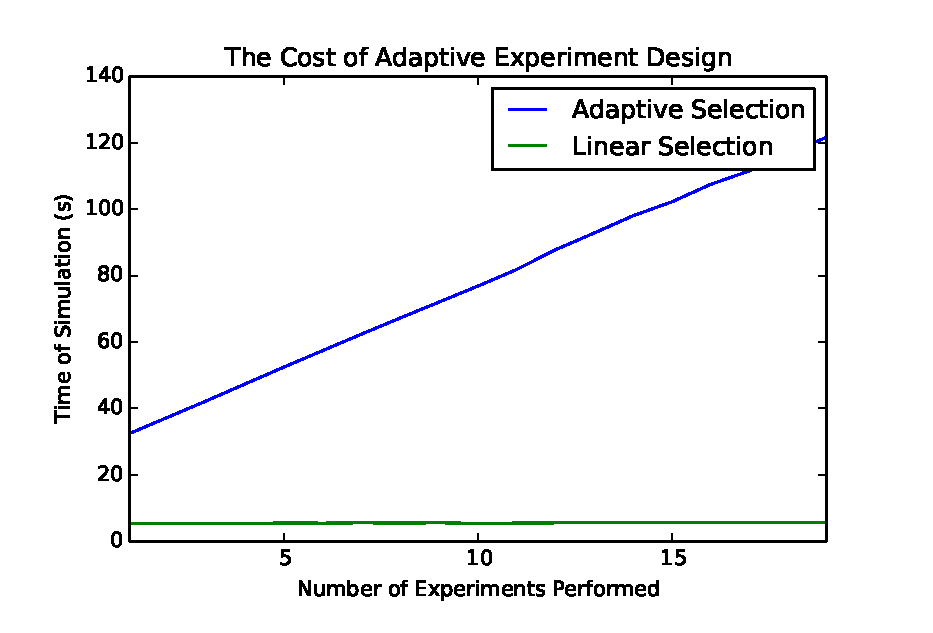
\includegraphics[scale=1.0]{Figures/adaptivetimes.eps}
\caption{The time of experiment simulation based on the number of experiments.}
\label{fig:adaptivetimes}
\end{figure}

It is also prudent to explore the behaviour of region estimation as described in section (\ref{sec:regionestimation}). The probability densities from parameter set one are seen in (\ref{fig:probdensities}). It can be seen that all of the densities appear to be highly peaked and approximately normally distributed as expected. This provides strong evidence that region estimation is functioning as anticipated. 

 \begin{figure}[ht!]
\centering
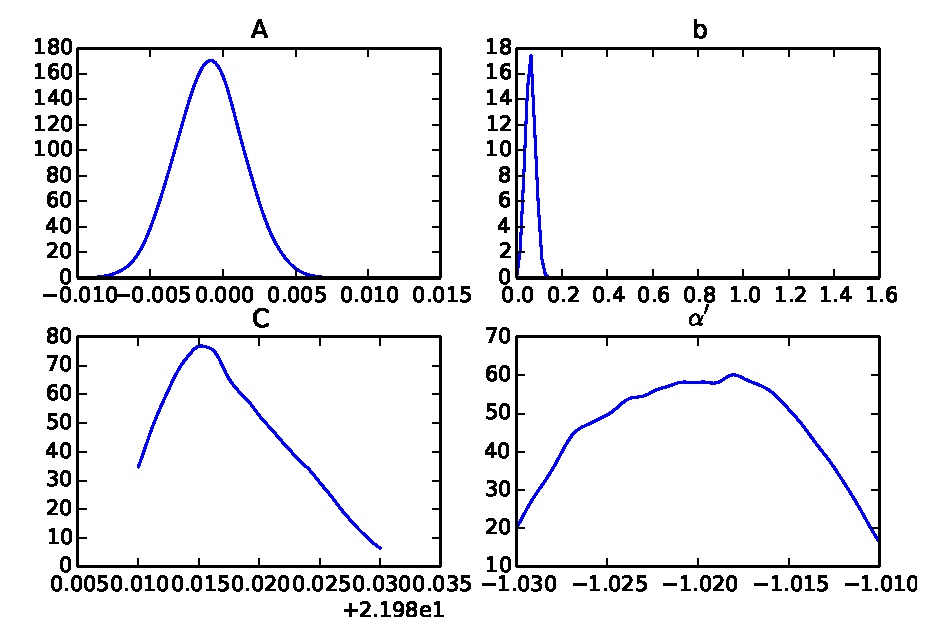
\includegraphics[scale=1.0]{Figures/probdensities.eps}
\caption{Probability density distributions of Bayesian estimators for the system parameters}
\label{fig:probdensities}
\end{figure}